\uuid{Ydt9}
\exo7id{1517}
\auteur{barraud}
\organisation{exo7}
\datecreate{2003-09-01}
\isIndication{false}
\isCorrection{false}
\chapitre{Endomorphisme particulier}
\sousChapitre{Endomorphisme du plan}

\contenu{
\texte{
Dessiner l'allure du Shadock ci dessous après qu'il ait subi l'action de
l'endomorphisme de $\R^{2}$ dont la matrice dans la base canonique est

$$
A=
\begin{pmatrix}
 1/2 & 0\\
  0 & 2  
\end{pmatrix}
\quad
B=
\begin{pmatrix}
  1 & 1/2\\
  0 & 1  
\end{pmatrix}
\quad
C=
\begin{pmatrix}
  0 & 1\\
  1 & 0  
\end{pmatrix}
\quad
D=
\begin{pmatrix}
  1/2 &-\sqrt{3}/2\\
  \sqrt{3}/2 & 1/2  
\end{pmatrix}
\quad
E=
\begin{pmatrix}
   1   &-1\\
  -1/2 & 3/2  
\end{pmatrix}
$$

Ecrire la matrice de la dernière transformation dans la base
$((2,1),(-1,1))$.

$$
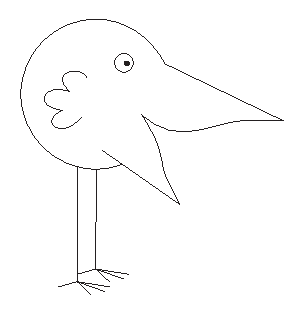
\includegraphics{../images/img001517-1}
$$
}
}
